\documentclass[11pt,letterpaper]{article}
\usepackage[margin=1in]{geometry}
\usepackage[T1]{fontenc}
\usepackage{lmodern,microtype,amsmath,amssymb,booktabs,longtable,array,graphicx,xcolor}
\usepackage[colorlinks=true,linkcolor=blue!45!black,citecolor=blue!45!black,urlcolor=blue!45!black]{hyperref}
\usepackage{url}
\urlstyle{same}
\setlength{\emergencystretch}{3em}
\setlength{\parskip}{0.25em}
\newcommand{\ev}[1]{\hyperref[app:evidence]{[E#1]}}
\newcommand{\code}[1]{\texttt{\detokenize{#1}}}
\title{Exact Storage, Inexact Recall:\\An Empirical Study of Disk-Backed Sparse KV Memory\\for Frozen Language Models}
\author{Josiah Wilson\\\small Independent research\\[0.5em]
\small AI research and laboratory assistance: Codex (OpenAI)\\
\small Astra, High reasoning; delegated GPT-6.1 Terra subagents}
\date{November 5, 2026\\\small Research manuscript, version 1.0; not peer reviewed}
\begin{document}
\maketitle
\begin{abstract}
Can a frozen language model retain a small active key--value (KV) cache while recovering distant information from an exact archive on disk? We investigate this question through a sequence of implementation checks, retrieval experiments, and cost measurements. Seven checkpoints from Qwen2.5, Qwen3, and SmolLM2 are explored, followed by reasoning and memory studies with a Qwen3 4B checkpoint. Model experiments cover nominal budgets from 4K to 32K tokens where supported. The prototype preserves exact archived KV for the trajectory that produced it, but approximates attention by selecting a subset of positions. In a Qwen2.5-1.5B confirmation, neighboring-block retrieval answers 24/30 factual cases versus 30/30 for a custom dense control. At 32K it answers 6/12 versus 12/12, while steady forced decoding averages 75.41 versus 148.56 ms per token for native stock inference. A separate matched teacher-forced experiment finds that an attention-based device reranker still takes 52.668 s versus 10.079 s for stock serving at 32K. In the final Qwen3-4B memory screen, the address-memory condition scores 6/10 versus 4/10 without memory at 32K, versus 10/10 for the full-cache control; initialized-cache request means are 45.242 and 78.673 s for addresses and full cache, respectively. These are small, correlated cohorts with different timing scopes, not pooled estimates. A tensor-checked diagnostic further shows an incorrect sparse answer despite retaining exact target-record KV, with exact logit and token recovery after restoring all archived KV in that trajectory. The tested implementations demonstrate useful memory and finite-range decoding tradeoffs, but not the joint target of near-full quality and lower complete-request cost. We provide a source-linked evidence ledger, disclose failed and canceled stages, and analyze why exact storage, successful retrieval, and successful use of retrieved context are distinct requirements.
\end{abstract}

\section{Introduction}
Autoregressive transformers reuse historical keys and values to avoid recomputing the entire prefix at each generated token. Dense decoding nevertheless attends over an expanding history. For long archives, storing and consulting that history can become a substantial memory and latency cost. The motivating proposal in this work is a small active memory in RAM or accelerator memory, supplemented by precise long-term KV on disk. Only the historical positions needed for a current computation should enter attention. Short-context overhead is acceptable if the system eventually offers substantially lower long-context latency with little loss in answer quality.

This proposal has two separate ambitions. The first is a bounded active attention set. The second is reliable access to useful information regardless of archive size. Achieving the first does not establish the second, and neither alone establishes a faster system. A retrieval engine can return the correct document while the model still fails to use its retained KV; an accurate selector can also cost more than the dense attention it replaces.

We evaluate a concrete training-free prototype rather than claim a new general solution to long-context inference. Related systems already investigate attention-aware vector retrieval, page selection, external context memory, and selective retention of attention heads \cite{liu2024retrievalattention,chen2025retroinfer,tang2024quest,xiao2024infllm,xiao2024duoattention}. Our contribution is a documented empirical investigation of a particular disk-backed implementation, including unsuccessful variants and controls that separate storage correctness, retrieval coverage, model behavior, and serving cost.

The investigation evolved from a single-model pilot into cross-model screening, held-out-seed confirmations, mechanistic controls, and separately frozen reasoning and memory cohorts. It was not a single globally preregistered benchmark. We preserve that distinction: post-hoc diagnostic cases are not presented as unseen confirmation, repeated timings do not increase the quality sample size, and an interrupted run is not silently converted into a successful run.

The principal findings are: (1) selected sparse policies reduce allocated CUDA memory and show roughly similar steady-decode times across the measured budgets; (2) factual accuracy can degrade even when all target-record positions are selected; (3) moving reranking to the GPU improves the tested CPU implementation but does not make that serving path competitive with stock; and (4) additional retrieval rounds and bounded remembered state provide selective recoveries, not general quality preservation. These are conclusions about the tested configurations. They do not prove that disk-backed sparse KV architectures cannot work.

\section{Related work and scope of contribution}
RetrievalAttention uses attention-aware vector retrieval for CPU-resident historical KV, addressing the mismatch between attention queries and a conventional vector index \cite{liu2024retrievalattention}. RetroInfer treats KV as vector storage and combines indexing with memory placement and transfer management \cite{chen2025retroinfer}. Both precede the general idea of fetching selected historical KV instead of retaining all of it in active accelerator memory. We do not claim priority for that idea.

Quest estimates query-dependent page importance from key extrema, enabling selective access to KV pages \cite{tang2024quest}. Our later diagnostic path uses page bounds and candidate reranking inspired by this family of methods, but is not a faithful reproduction of the complete Quest implementation. InfLLM retrieves relevant context-memory units without additional training \cite{xiao2024infllm}; our scope is primarily within the tested native context budgets, not extrapolation beyond them. StreamingLLM retains initial attention sinks and recent tokens to stabilize bounded-cache streaming \cite{xiao2023streamingllm}. Initial-token retention is relevant to our controls, but stable streaming does not itself recover an arbitrary forgotten fact. DuoAttention allocates different KV retention strategies to retrieval and streaming heads \cite{xiao2024duoattention}, illustrating that a uniform policy across heads is not the only design choice.

These methods motivate design alternatives and delimit novelty. None is a measured head-to-head baseline here. Their published speedups cannot be compared directly to our numbers because models, hardware, kernels, workloads, memory placement, and measurement boundaries differ. This paper reports an implementation study and its failure modes, not superiority over published retrieval-attention systems or an exhaustive review of all sparse-attention methods.

\section{Architecture and analytical model}
\subsection{Exact archive and bounded active view}
Let $N$ denote the number of archived positions, $L$ the number of layers, $H_{kv}$ the KV-head count, $d$ the head dimension, and $s$ the bytes per scalar. Uncompressed historical KV storage is approximately
\begin{equation}
M_{archive}(N)=2NLH_{kv}ds.
\end{equation}
The factor two accounts for keys and values. This payload estimate assumes one sequence, uniform layer dimensions and scalar width, and excludes padding, metadata, and filesystem overhead. An exact disk archive therefore grows with $N$ even if accelerator residency does not. ``Exact'' refers to the saved tensors for the computation that created them. KV produced by sparse online ingestion need not equal KV produced by a dense prefix computation.

The prototype stores unexpanded per-layer KV in binary files and maintains original absolute positions and rotations. A recent exact window, selected archive blocks, and, in early variants, compressed summaries form one attention view. Explicit causal masks use source positions rather than inferring position from the length of the assembled cache. Different study stages use different policies; there is no single selector that produced every result in this paper.

The reasoning and memory experiments disable compressed KV ($C=0$), use a recent window $W=2000$, retain 128 initial positions, and select at most sixteen 128-token blocks. The configured maximum active view is thus 4176 entries; underfilling and overlap can reduce actual counts. Source-text metadata returns block addresses. The original per-layer KV at those addresses is loaded for attention. Retrieved source text is not inserted into the prompt. In the memory-harness experiments, model-generated notes are inserted, making those variants explicitly hybrid KV-plus-text-memory systems.

The initial pilot instead includes compressive state and a head-averaged, post-rotation query versus page-centroid cosine selector. That selector scans candidates linearly; calling it an approximate-nearest-neighbor index would misdescribe the implementation. Later SQL-backed text selectors and attention-based rerankers are separate branches of the investigation.

\subsection{Index and selection variants}
The text index uses SQLite tables for block addresses, token ranges, text metadata, postings, and embedding vectors. SQL storage and retrieval-augmented KV attention are complementary, not competing designs. Actual KV remains in binary archive files. Tested selectors include lexical ranking, capped rare-term candidates, neighboring-block expansion, exact semantic-vector scans, and semantic reranking. The bounded rare-term path reads a capped candidate list for a distinctive query term; it cannot guarantee semantic recall when such a term is absent. An exact vector scan remains linear in the number of indexed blocks.

The later attention path uses current attention queries to rank candidate pages and then evaluates candidate keys more directly. The tested reranker selects 32 candidate pages and up to 15 final pages, subject to eligibility and active-memory rules. A device implementation reduces CPU/device movement during scoring, but retains a CPU metadata scan. Correctly reproducing that selector on device does not establish an efficient asymptotic index. The memory and reasoning cohorts use the earlier text-index policy, not this later attention reranker.

\subsection{Why exact selected KV can still yield an inexact answer}
For one fixed attention head, write dense attention as
\begin{equation}
o=\sum_{i=1}^{N}p_i v_i,\qquad p_i=\frac{\exp(q^\top k_i/\sqrt d)}{\sum_j\exp(q^\top k_j/\sqrt d)}.
\end{equation}
For this counterfactual calculation, keep the query, keys, values, allowed positions, and logits identical before removing positions. If a nonempty subset $S$ is retained, subset attention renormalizes the retained weights. Let $m=\sum_{i\notin S}p_i$ be the omitted dense mass. For $0<m<1$, let $o_S$ and $o_O$ be the normalized retained and omitted outputs. Then
\begin{equation}
o=(1-m)o_S+mo_O,\qquad o_S-o=m(o_S-o_O).
\end{equation}
If all values have norm at most $V$, this gives $\|o_S-o\|\leq 2mV$. This is an elementary one-head, fixed-query calculation, not an empirical error bound for our full model. Subsequent layers and tokens can change their queries after an earlier approximation. Importantly, retaining a semantically relevant fact does not ensure that the omitted attention mass is small, nor that the omitted values are unimportant to the computation. Exact storage alone cannot guarantee exact behavior.

\subsection{Cost boundaries}
With a fixed active budget $B$, attention over that budget can avoid direct dependence on $N$. Complete work still contains other terms:
\begin{equation}
T_{step}(N,B)=T_{lookup}(N)+T_{fetch}(N,B)+T_{model}(B)+T_{bookkeeping}.
\end{equation}
This is an illustrative accounting model, not a fitted performance law. $T_{model}(B)$ abbreviates the fixed-model computation with bounded active attention; it is not a claim that all implementation costs depend only on $B$. Archive construction, index construction, verified mounting, and checkpoints are additional costs. Even a bounded candidate count does not imply bounded lookup time if discovering candidates scans metadata. A fixed GPU KV budget likewise says nothing by itself about CPU index memory, the filesystem cache, or transient buffers. Newly ingesting $N$ tokens requires processing those tokens at least once; our target concerns subsequent access and generation, not free ingestion. More reasoning rounds add model and retrieval work and must be charged explicitly.

\section{Experimental methods}
\subsection{Models, environment, and controls}
Model execution used one Colab Tesla T4 at a time, frozen fp16 weights, batch size one, and greedy generation. The recorded environment includes Python 3.13.16, PyTorch 2.6.0+cu124, Transformers 4.51.3, NumPy 2.2.4, and Hugging Face Hub 0.30.2. Seven exploratory checkpoints comprise Qwen2.5-Instruct 0.5B/1.5B/3B, Qwen3 0.6B/1.7B, and SmolLM2-Instruct 360M/1.7B. Qwen3-4B-Instruct-2507 is evaluated separately in the reasoning and memory cohorts. Names are nominal size labels, not substituted measurements of loaded parameters. Exact model revisions are recorded in the manifests and Appendix~\ref{app:models}.

Model studies cover nominal 4K, 8K, 16K, and 32K budgets as applicable; SmolLM2 studies stop at 8K. Not every model is tested in every cohort or at every length. The reasoning protocols reserve 2048 tokens, so their 8K/32K labels correspond to archives of approximately 6K/30K, with actual token counts saved per fixture. Synthetic index-only tests above native lengths are explicitly not model evaluations.

We distinguish three full-cache baselines. \emph{Native stock HF} is the practical dense timing control without sparse archive writes. \emph{Custom full-buffered} is an implementation-matched dense policy used in factual and online comparisons. \emph{Stock in archive-session studies} executes full attention after loading a shared immutable archive, and is not identical to a continuously resident vanilla deployment. Tables identify which applies. A parity test at one schedule is not a license to substitute these baselines everywhere.

\subsection{Implementation checks}
The initial five CUDA gates passed before the pilot. A prior chunked-prefill discrepancy of 0.01953125 was also observed in vanilla fp16 execution under different shapes; matched-schedule controls retained their stringent tolerance rather than declaring a mask bug from cross-schedule rounding alone. Subsequent snapshots checked masks, positions, grouped-query attention, fixed-policy resume, and source/runtime identity. For example, the Qwen1.5 confirmation reports zero logit error in its matched-schedule controls and bit-identical resumed KV \ev{1}.

Validation remains scoped. An older validation path silently skipped a custom \code{full_buffered} name; the defect and corrected snapshot are recorded instead of retroactively assigning new validation to old results. The device reranker underwent numerical replay and tiny-model integration checks before matched cost tests. Such checks establish specified implementation properties, not model quality, deployment robustness, or a replication by an independent laboratory.

\subsection{Tasks and study sequence}
The pilot preserves 95 completed records from an originally planned 255-row matrix. Follow-up demand retrieval comprises a 123-row first study, a 68-row ablation, and a 489-row seven-model screen. These counts are execution records, including policies and repetitions, not independent examples \ev{15}. Subsequent confirmations freeze new seeds and compare factual recall at several depths, many-key distractors, literal questions, and paraphrases. Qwen1.5 and Qwen3 confirmations each contain 264 records: 180 factual policy observations and 84 forced-timing observations. Their 30 factual cases reuse targets across lengths. SmolLM2-1.7B has a separate 150-record confirmation with 18 factual cases \ev{1}\ev{2}\ev{3}.

Persistent-session and tensor-restoration controls investigate whether failures reflect missing records or insufficient context despite record retention. Later attention-reranker studies separate reused-case tuning, fixed-policy transfer, and matched cost. No oracle or gold answer is used to choose the final ordinary policy's output. Oracle-style diagnostics are labeled as such and excluded from general performance claims.

Each reasoning cohort contains eight seed/task questions at two lengths, eleven policy configurations, and extra timing repetitions: 176 quality observations plus 44 additional timing observations, or 220 rows. Tasks include literal recall, paraphrase, a linked-record lookup, and addition over separated records. Models produce structured answers, retrieval queries, and short notes; subsequent retrieval uses the generated search field, with a declared fallback for invalid queries. One, two, or four rounds have 128-token per-round caps. Additional one- and two-round variants use 512 and 256 token caps, respectively, to compare equal maximum generated-token allowances. Caps are not equal realized work. All rounds execute and the final draft is scored, rather than selecting the best draft with ground truth \ev{7}\ev{8}.

Each memory cohort contains four archive episodes, each with five sequential questions: two episodes at each of the two lengths. The lengths and policies reuse question structure and facts. Six natural-memory policies produce 120 observations; two explicitly stale-note policies add 40. Every policy receives two 128-token rounds. Only declared bounded notes and/or addresses persist between otherwise fresh question sessions; archive facts are not appended during these tests. The stale-note arm injects an obsolete note as a stress condition, not as a claimed earlier model output \ev{9}\ev{10}.

\subsection{Metrics, timing, and inferential limits}
Accuracy follows each frozen task scorer. Exact final answers, code presence in prose, and successful JSON parsing are different outcomes. We do not pool them. The all-KV diagnostic uses correct-code presence and full token/logit comparisons; the structured reasoning and memory tables use their declared exact-answer scorer. A format failure is retained as a primary failure even when a post-hoc reading finds a code in the output.

Steady forced-decode timing excludes retrieval setup and other lifecycle costs in the confirmation experiments. Initialized-cache request timing includes question/review prompts, lookups, and generated drafts but excludes mounting, controller initialization, shared prefix/index preparation, and checkpointing. The matched reranker cost experiment times a fixed prompt plus 64 teacher-forced steps with identical inputs across arms within each length. Separately reported ``accounted service'' sums component timers; it is not one continuously measured wall interval. Native stock batches prompts, whereas sparse prompts are processed serially in these implementations. Instrumentation and periodic result backup can add overhead.

CUDA allocated peaks are framework allocations, not all device-resident memory. Host RSS is process memory, not whole-system RAM. Store-read bytes are logical reads, not measured physical SSD traffic. OS cache conditions were not controlled. The Colab filesystem is therefore described as disk-backed storage, without inferring the behavior of a particular local SSD.

The study is descriptive. We do not report inferential confidence intervals from correlated policy rows or claim statistical equivalence. Three repetitions of one fixture estimate observed timing variation, not performance over a workload population. Sequential memory questions share state; length variants reuse facts; exploratory choices are adaptive. Reported ranges are observed ranges. Near-lossless generalization would require an adequately powered, independently sampled confirmation with a prespecified margin, which this investigation did not complete.

\section{Results}
\subsection{Steady decoding can flatten while factual quality falls}
Table~\ref{tab:confirm} summarizes the two Qwen confirmations. The sparse policy is rare-term selection with neighboring context (\code{rare-context} in saved reports). Quality uses the custom dense control; timing compares native stock HF. In Qwen1.5 all 18 ordinary 4K/8K/16K cases are answered by the indexed policies, but neighboring retrieval falls to 6/12 at 32K against dense 12/12. The larger case mix at 32K precludes interpreting the overall accuracy change as a clean length-only intervention. Four neighboring-policy failures retain the entire target record's positions; two paraphrase failures omit it \ev{1}.

\begin{table}[ht]
\centering\small
\begin{tabular}{lrrrr}
\toprule
 & \multicolumn{2}{c}{Qwen2.5-1.5B} & \multicolumn{2}{c}{Qwen3-0.6B}\\
Measure & Dense/stock & Sparse & Dense/stock & Sparse\\\midrule
All factual cases & 30/30 & 24/30 & 26/30 & 24/30\\
32K factual cases & 12/12 & 6/12 & 8/12 & 7/12\\
32K decode (ms/token) & 148.56 & 75.41 & 209.62 & 85.29\\
32K CUDA peak (GiB) & 3.946 & 2.969 & 4.87 & 1.42\\\bottomrule
\end{tabular}
\caption{Separate confirmation cohorts \ev{1}\ev{2}. Accuracy: custom full-buffered dense versus sparse. Timing: native stock HF versus sparse, means from three forced-decode trials; setup and query processing excluded. CUDA values have the precision of the source reports. Cases are correlated across lengths; this is not a pooled benchmark.}\label{tab:confirm}
\end{table}

Qwen1.5 neighboring retrieval averages 79.18, 78.99, 79.45, and 75.41 ms/token at nominal 4K, 8K, 16K, and 32K, respectively. Native stock averages 37.30, 51.25, 84.70, and 148.56 ms/token. The observed crossing between the two middle budgets supports the intended finite-range decoding behavior. It does not establish constant complete-request cost. Stock runs last within these trials, and cache/setup effects remain potential confounds. In SmolLM2-1.7B, neighboring retrieval retains 15 of the dense control's 17 correct answers across 18 cases; at 8K it saves about 22\% allocated CUDA memory but decodes about 18\% more slowly, with all three paired trials slower \ev{3}. The speed tradeoff therefore differs by model and supported length.

\begin{figure}[ht]
\centering
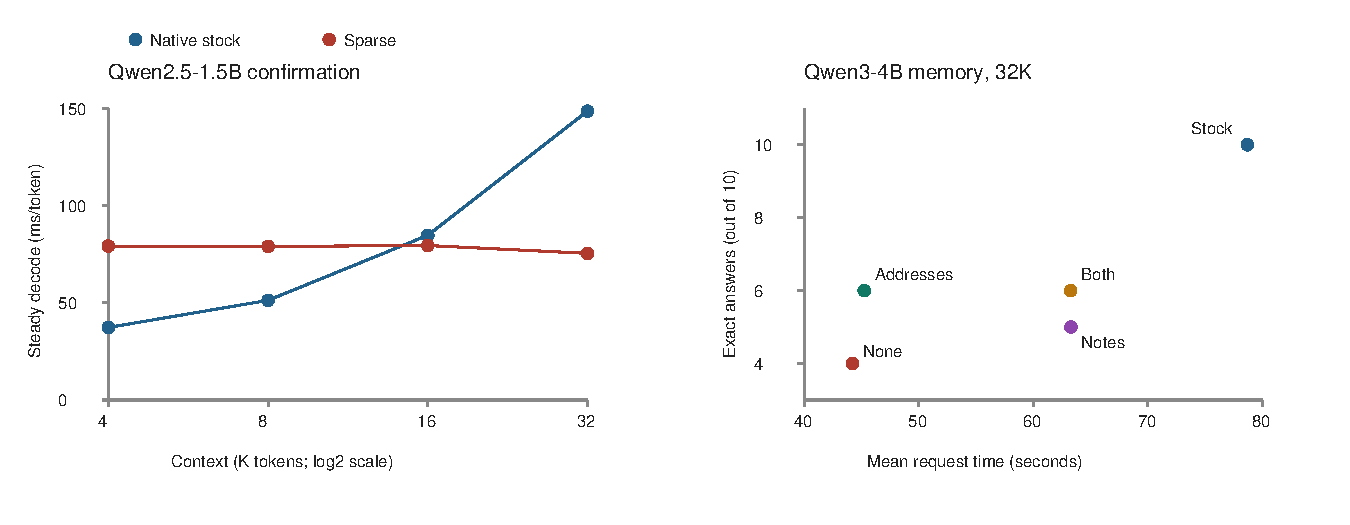
\includegraphics[width=\linewidth]{figure_tradeoffs.pdf}
\caption{Two distinct tradeoffs, not a joint benchmark. Left: Qwen1.5 confirmation means from three forced-decode trials per budget; lookup, query processing, and setup are excluded. Right: Qwen4 memory-screen mean initialized-cache request times and exact-answer counts at nominal 32K; ten correlated question observations per policy, variable outputs, no repeated timing trials. No confidence intervals are implied. Sources: \ev{1}\ev{10}.}
\label{fig:tradeoffs}
\end{figure}

\subsection{Retaining a fact is not sufficient in a tensor-checked case}
A persistent-session study produces 8/12 distinct correct answers for neighboring retrieval versus 11/12 for stock, losing all three 32K answers despite complete-record selection \ev{4}. A subsequent control reuses the first 32K failure, a 31,718-token prefix, the same question schedule, and the original checkpoint. It compares stock, the sparse view, and an all-KV view routed through the retrieval assembly path \ev{5}.

The sparse view contains the target record at all 28 layers; its actual archived keys and values match the disk tensors bit for bit. It still fails to state the correct code. Restoring all 248 archived blocks recovers all 24 question-token logit vectors exactly, with maximum absolute error zero, and all 23 generated token IDs, including EOS. This directly checks more than record-address coverage. It rules out a generic inability of this assembly path to reproduce dense attention on this trajectory. It does not identify the particular omitted positions responsible or establish the cause of every other error.

A post-hoc neighboring-budget sweep recovers three lost Qwen1.5 32K cases, raising the count from 6/12 to 9/12 with sixteen or thirty-two nearby blocks, still below dense 12/12 \ev{6}. Those recovered cases already had full target-record coverage at the smaller budget. A separate initial-token/sink diagnostic improves a reused set from 8/12 to 9/12 versus stock 11/12 \ev{16}. That comparison changes available context and is not an equal-budget causal estimate of an isolated sink mechanism.

\subsection{Attention reranking: implementation improvement, no serving win}
The matched cost experiment contains three balanced-order requests per arm per length, eighteen requests in total. Within a length, stock, CPU reranking, and device reranking receive the same 102 prompt tokens and 64 forced continuations. Untimed CPU/device checks cover 4,648 layer/position events per length, with matching routes, exact fp16 KV hashes, and maximum logit difference zero. Timed sparse route observations agree with their respective validation traces \ev{11}.

\begin{table}[ht]
\centering\small
\begin{tabular}{llrrrr}
\toprule
Budget & Arm & Prompt (s) & Forced (s) & Serving (s) & Step (ms)\\\midrule
8K & Native stock & 0.094 & 2.854 & 2.948 & 44.562\\
8K & CPU reranker & 29.819 & 18.174 & 47.891 & 283.926\\
8K & Device reranker & 23.387 & 14.524 & 38.102 & 226.913\\
32K & Native stock & 0.291 & 9.778 & 10.079 & 152.730\\
32K & CPU reranker & 37.509 & 23.731 & 61.092 & 370.768\\
32K & Device reranker & 31.889 & 20.854 & 52.668 & 325.811\\\bottomrule
\end{tabular}
\caption{Matched teacher-forced cost \ev{11}. Cells are medians of three repetitions; step values are medians of per-repetition mean synchronized step times. Component medians need not sum to serving medians. This is a fixed-work cost test, not an answer-quality result.}\label{tab:cost}
\end{table}

The median paired device/CPU serving ratios are 0.797 at 8K and 0.860 at 32K. Device/stock ratios are 12.889 and 5.237, respectively. Thus the port improves this CPU path but remains substantially slower than stock, including in the forced steps. At 32K, post-reset allocated CUDA peaks are approximately 3.083 GiB for device and 3.923 GiB for stock. Shared prefix construction, mounting, initialization, and checkpoints are outside the serving column. Different fixtures across lengths prevent attributing its entire cross-length change to archive size.

Instrumentation explains part of the cost. A separate twelve-request, device-only ablation reduces median serving time from 39.028 to 30.051 s at 8K and from 52.027 to 43.147 s at 32K when route/hash observation is disabled \ev{12}. There is no contemporaneous stock arm in this ablation. Timed-off routes were not recorded; untimed surrounding validations and final checks do not replace a missing timed trace. We therefore do not combine these numbers into a new controlled stock comparison.

Fixed-policy transfer also separates scoring from usefulness. In twelve Qwen1.5 fixtures, stock and reranker match correctness in both rounds, each scoring 4/6 at 8K and 3/6 at 32K. This low-accuracy agreement is not equivalence. Smol's structured-output transfer produces parser failure in all 24 round outputs across six fixtures and two arms, making a 0/6 versus 0/6 comparison uninformative about retained factual ability. A separately declared short-answer control with new fixtures scores 4/6 in both arms and rounds. Since prompts, fixtures, and output caps change together, it is not a format-only causal test \ev{17}.

\subsection{Additional reasoning and renewed retrieval}
Table~\ref{tab:reason} shows the nominal 32K reasoning screen for both models. Each retrieval round can use a model-generated search query; the active selection is replaced rather than accumulated without bound. Sparse active KV never exceeds 4176 entries in the saved reports.

\begin{table}[ht]
\centering\small
\begin{tabular}{lrrrr}
\toprule
 & \multicolumn{2}{c}{Qwen2.5-1.5B} & \multicolumn{2}{c}{Qwen3-4B}\\
Policy at 32K & Exact & Request (s) & Exact & Request (s)\\\midrule
Stock direct & 4/8 & 1.221 & 6/8 & 4.619\\
Stock JSON, 1 round & 4/8 & 9.943 & 6/8 & 44.937\\
Stock JSON, 2 rounds & 5/8 & 22.424 & 7/8 & 86.138\\
Stock JSON, 4 rounds & 5/8 & 47.254 & 7/8 & 182.263\\
Sparse JSON, 1 round & 2/8 & 11.510 & 2/8 & 21.918\\
Sparse JSON, 2 rounds & 2/8 & 27.809 & 2/8 & 46.442\\
Sparse JSON, 4 rounds & 2/8 & 56.846 & 3/8 & 100.179\\\bottomrule
\end{tabular}
\caption{Reasoning screen \ev{7}\ev{8}: 128 generated-token cap per round; mean initialized-cache request seconds over eight questions per cell, including failures. These are realized variable-length outputs. Stock uses the shared archive-session baseline. Rows and lengths are correlated.}\label{tab:reason}
\end{table}

For Qwen1.5, extra sparse rounds recover no additional answers at either length, while increasing time. For Qwen4, four sparse rounds raise accuracy from 3/8 to 5/8 at 8K and from 2/8 to 3/8 at 32K. At 32K, matching four-round stock answers 7/8; even direct stock answers 6/8 much sooner. The four-round sparse mean changes little between 8K and 32K (99.818 to 100.179 s), but the quality difference prevents interpreting that flatness as successful replacement of full attention. One- and two-round variants with the same maximum total token allowance of 512 do not recover further sparse answers in these cohorts. Maximum allowances and actual generated/evaluated tokens remain distinct.

The Qwen4 worker finishes all 220 rows, but its controller exits with a finalization error after counting an unrelated bundled directory as a run directory. Worker success, controller failure, and recovered artifact checks are all retained \ev{8}. Earlier out-of-memory and partial attempts are not pooled with the successful worker cohort. This distinction is necessary for interpreting both completion and operational reliability.

\subsection{Bounded notes and remembered addresses}
The final Qwen4 memory experiment completes all 160 scheduled rows with successful worker and controller exits. Table~\ref{tab:memory} presents all natural-memory policies. Both sparse and stock receive the same two-round opportunity. The address-only variant avoids inserting notes but reuses a bounded list of previously selected archive addresses.

\begin{table}[ht]
\centering\small
\begin{tabular}{lrrrrrr}
\toprule
 & \multicolumn{3}{c}{8K nominal} & \multicolumn{3}{c}{32K nominal}\\
Policy & Exact & Time (s) & GiB & Exact & Time (s) & GiB\\\midrule
Stock, none & 10/10 & 19.765 & 8.506 & 10/10 & 78.673 & 12.256\\
Stock, notes & 10/10 & 23.027 & 8.548 & 10/10 & 86.115 & 12.299\\
Sparse, none & 5/10 & 46.912 & 8.174 & 4/10 & 44.217 & 8.174\\
Sparse, notes & 7/10 & 63.830 & 8.174 & 5/10 & 63.278 & 8.174\\
Sparse, addresses & 6/10 & 46.820 & 8.174 & 6/10 & 45.242 & 8.174\\
Sparse, both & 6/10 & 64.425 & 8.174 & 6/10 & 63.263 & 8.174\\\bottomrule
\end{tabular}
\caption{Qwen3-4B natural-memory screen \ev{10}. Time is mean initialized-cache request duration; GiB is allocated CUDA peak. Ten question observations per cell arise from two five-question episodes at each length. There are no repeated timing trials. Archive preparation and mounting are excluded.}\label{tab:memory}
\end{table}

At 32K, the saved-address condition scores 6/10 versus 4/10 without memory, with a request mean of 45.242 s versus stock's 78.673 s, but stock answers all ten. At 8K, address memory gives 6/10 versus stock 10/10 and is slower. Notes cost more and do not outperform addresses at 32K. This is a useful memory mechanism on some questions, not a quality-preserving speedup. In the separate Qwen1.5 memory cohort, addresses raise 32K sparse accuracy from 3/10 to 5/10, matching stock's count but not its set of successes. Its mean is 27.039 s versus stock 25.061 s \ev{9}.

The Qwen4 stale-note stress yields 10/10 for stock notes and 6/10 for sparse combined memory at both lengths. These injected stale notes are not natural model mistakes. Observed memory-state maxima are 245 stored text tokens, 256 memory-prompt-body tokens before serialization, and twelve address integers. Complete serialized prompts are counted separately. These logical bounds do not establish constant host RSS or index size. Neither memory cohort tests newly appended facts or an uninterrupted long-running KV conversation. Planned update cohorts for both models were canceled before execution; cancellation is not a negative experimental result.

\subsection{Index scaling, ingestion, and other boundary checks}
Synthetic CPU indexing isolates a remaining cost. A page-bound scan across 28 layers takes a median 8.218 ms for 32,768 represented positions and 158.846 ms for 1,048,576, using seven warm trials per size. At the latter size, metadata occupies 471,597,056 bytes and sampled process peak RSS is 981,172,224 bytes \ev{13}. The test excludes model inference, real historical KV construction, GPU transfer, and disk reads. It demonstrates growth in this specific scan, not million-token inference or a prediction of T4 latency.

Three empty-start online cohorts, each with nine observations, test Qwen1.5, Qwen3-0.6B, and SmolLM2-1.7B on three layouts of one reused target association. Sparse ingestion is slower in the recorded comparisons and can use less CUDA memory; the dense control itself writes to disk. Index metadata is prebuilt, so these runs do not demonstrate an incremental bounded-memory index. Sparse online KV is exact for its own trajectory, not promised identical to dense ingestion \ev{18}.

A two-document summary study contains twelve observations and mixed coverage and factual errors in both sparse policies and a custom dense control. Its source-based assessment is by a single policy-visible reviewer, not a blinded or independent human benchmark evaluation \ev{19}. It is insufficient to generalize from synthetic recall to reliable long-document summarization. These boundary studies are preserved because they limit, rather than expand, the main positive claims.

\section{Discussion}
\subsection{Three distinct bottlenecks}
The data motivate separating \emph{candidate recall}, \emph{context sufficiency}, and \emph{execution cost}. Paraphrase failures can be retrieval misses. Exact target-record retention followed by an incorrect answer shows that a different class of failure remains after that particular miss is eliminated. Finally, the attention reranker matches stock's correctness on a small transfer set while the separate matched-cost study shows a serving slowdown. This agreement does not imply identical outputs or general behavioral preservation. A faster database alone addresses only part of this chain.

The tensor-restoration result supports context dependence beyond a single target record, but does not establish one universal ``utilization wall.'' Possible contributors include omitted attention mass, surrounding contextual representations, head-specific selection, positional effects, and trajectory divergence. The one-head calculation explains why exact subset tensors do not mathematically guarantee dense behavior; it does not identify which mechanism dominates the experiments. A strong causal claim would require additional interventions, which are outside this closed study.

\subsection{What the cost evidence establishes}
The most favorable decode results and the unfavorable reranker request results are not contradictory. They measure different policies and different parts of serving. Text-index policies can select once and reuse a small working set during decoding, while attention-based selection repeatedly pays search and movement costs. Sparse prompt execution is also serial in this prototype. Improving batching, storage locality, candidate reuse, and query-aware indexing could change results, but this paper does not report those unmeasured improvements as achieved.

The desired advantage at very large archive sizes remains plausible as a design objective, not demonstrated here. Fixed active attention can remove a direct linear term while leaving linear index scans, ingestion, mounting, or memory growth elsewhere. The present maximum model budget is 32K. Extrapolating a flat curve to one million tokens would ignore native position support, retrieval recall, representation drift, and the metadata costs already visible in the synthetic scan.

\subsection{Implications for future designs, not new results}
Several directions follow from the observed failures and prior work. Query- and head-aware retrieval could preserve more relevant attention mass than semantic source matching alone. Keeping initial sinks and selected surrounding context may help stabilize a sparse view, but should be tested under matched budgets. A graph or hierarchical index with explicit search-work limits could replace the full metadata scan, while reporting the resulting recall tradeoff. Candidate caching and grouped disk access could reduce repeated transfer. A memory harness could retain reliable address associations and query reformulations, while treating generated notes as fallible and charging their token cost.

These proposals would need separate experiments; none is a validated resolution of the bottleneck. More retrieval rounds are particularly not a free remedy: their usefulness depends on generating a better query or retaining a useful intermediate state, and the measured smaller-model cohort recovered no extra answers. Any future success criterion should combine task quality and total measured cost at the same workload, with component costs and amortization assumptions stated explicitly.

\section{Limitations and threats to validity}
\paragraph{Sampling and adaptation.} The study uses small synthetic factual cohorts, reused targets and templates, correlated episode sequences, and a small number of natural documents. Screening and post-hoc tuning are adaptive. Held-out seeds reduce one source of reuse but do not create a representative task distribution. No broad quality-equivalence claim, statistical significance claim, or estimated population-wide loss rate is justified.

\paragraph{Systems comparison.} All model execution uses a single class of T4 GPU in a managed runtime. Runtime replacement, allocator behavior, OS caching, output length, prompt batching differences, and instrumentation influence timing. Some measurements are forced fixed work; others are variable-output task means. Some costs are excluded, shared, or summed from separate timers. They cannot be pooled into one end-to-end speedup. There is no measured physical-SSD deployment, concurrency scaling test, power study, or inference at one million tokens.

\paragraph{Model and policy scope.} The tested checkpoints span multiple sizes but only the stated families and adapters, without training or weight quantization. Not every variant runs on every checkpoint. The original compressive-memory design, text-index policies, attention reranker, and note harness are distinct implementations. Generalizing results from one to all of them would be invalid. Dense and sparse online histories need not produce identical KV.

\paragraph{Measurement and provenance.} Saved output replay, hash checks, and source audits establish consistency with recorded artifacts, not that independent operators reproduced the experiments on another machine. Some large payloads remain in private Drive rather than the Git repository. Hash-only route evidence cannot reconstruct raw tensors. The memory runner asserts the parameter count live but does not persist it separately in its validation JSON. Raw normalization values for one numerical replay were not retained. Failed and incomplete attempts remain separate and are not counted as successful observations.

\paragraph{AI-mediated execution and review.} AI agents implemented and operated much of the study, scored or checked artifacts, and drafted this paper. Separate-agent checks can share assumptions, source code, and systematic errors. They are not equivalent to independent human review. The manuscript preparation pass checks saved evidence without rerunning models; it cannot guarantee that every latent implementation error has been found. Human author review and external scientific scrutiny remain necessary before submission.

\section{Conclusion}
The tested disk-backed sparse KV prototype achieves lower accelerator allocations and flatter steady decoding in some finite-context settings, but does not demonstrate the joint objective of near-full answer quality and lower complete-request cost. Exact target-record KV can be present without preserving the dense answer; additional context can repair some failures, and restoring all archived KV exactly recovers the saved question logits and output tokens in one tensor-checked trajectory. The tested attention-based reranker incurs substantial overhead. Bounded notes, addresses, and repeated retrieval recover some answers but do not close the general quality gap. The central empirical lesson is to evaluate storage fidelity, retrieval sufficiency, and whole-request efficiency separately, then require them to succeed together.

\section*{Contributions, acknowledgments, and AI assistance}
Josiah Wilson originated the project-specific architectural proposal and objectives, supplied the computing and service resources, directed the scope and research priorities, and decided when to end experimentation. This attribution concerns this project; it is not a claim of priority over the related literature.

Codex (OpenAI) served as an AI research and laboratory assistant for implementation, experiment operation, diagnostics, evidence preservation, literature review, analysis, and manuscript drafting. At the author's request, the principal assistant is identified as \emph{Astra at High reasoning}, with \emph{GPT-6.1 Terra subagents} used for delegated implementation and audit work, including the manuscript evidence and literature checks. The principal-assistant configuration is author-specified attribution, not a setting independently recorded in every experimental manifest. The record also includes earlier coordination and handoff assistance attributed to Muse/Orion; exact model identities for every historical interaction are not asserted.

AI assistance is disclosed as assistance, not a separate human author or an independent laboratory. No independent human replication or peer review has occurred as part of manuscript preparation. Before public submission, the human author must review and accept responsibility for the claims, sources, disclosures, and applicable venue requirements. Resources were provided by the author; no external grant award is asserted. No new model experiments were performed to prepare this manuscript.

\section*{Data and code availability}
The public artifact package is \href{https://github.com/Aperturesurvivor/tiered-kv-cache-research/tree/v1.0.0}{Aperturesurvivor/tiered-kv-cache-research, version 1.0.0}. Appendix~\ref{app:evidence} maps claims to retained artifacts. The completed-study source snapshot \texttt{735155ba7db1828ffb737\allowbreak 0c2ae354cb008a6908f} and earlier run revisions identify private source provenance, not commits in this public repository. Saved observations support recomputation of the four principal tables; preserved logits support the all-KV comparison. Other claims have selected report-level evidence and varying raw support, not full replay. Some operational records and large payloads are omitted. See the release manifest for scope and transformations. Model and dataset access and license requirements remain separate.

\begin{thebibliography}{9}
\bibitem{liu2024retrievalattention} Liu, Di, Chen, Meng, Lu, Baotong, Jiang, Huiqiang, Han, Zhenhua, Zhang, Qianxi, Chen, Qi, Zhang, Chengruidong, Ding, Bailu, Zhang, Kai, Chen, Chen, Yang, Fan, Yang, Yuqing, Qiu, Lili. RetrievalAttention: Accelerating Long-Context LLM Inference via Vector Retrieval. arXiv:2409.10516, 2024. \url{https://arxiv.org/abs/2409.10516}.

\bibitem{chen2025retroinfer} Chen, Yaoqi, Zhang, Jinkai, Lu, Baotong, Zhang, Qianxi, Zhang, Chengruidong, Luo, Jingjia, Liu, Di, Jiang, Huiqiang, Chen, Qi, Liu, Jing, Ding, Bailu, Yan, Xiao, Jiang, Jiawei, Chen, Chen, Zhang, Mingxing, Yang, Yuqing, Yang, Fan, Yang, Mao. RetroInfer: A Vector-Storage Approach for Scalable Long-Context LLM Inference. arXiv:2505.02922, 2025. \url{https://arxiv.org/abs/2505.02922}.

\bibitem{tang2024quest} Tang, Jiaming, Zhao, Yilong, Zhu, Kan, Xiao, Guangxuan, Kasikci, Baris, Han, Song. Quest: Query-Aware Sparsity for Efficient Long-Context LLM Inference. arXiv:2406.10774, 2024. \url{https://arxiv.org/abs/2406.10774}.

\bibitem{xiao2024infllm} Xiao, Chaojun, Zhang, Pengle, Han, Xu, Xiao, Guangxuan, Lin, Yankai, Zhang, Zhengyan, Liu, Zhiyuan, Sun, Maosong. InfLLM: Training-Free Long-Context Extrapolation for LLMs with an Efficient Context Memory. arXiv:2402.04617, 2024. \url{https://arxiv.org/abs/2402.04617}.

\bibitem{xiao2023streamingllm} Xiao, Guangxuan, Tian, Yuandong, Chen, Beidi, Han, Song, Lewis, Mike. Efficient Streaming Language Models with Attention Sinks. arXiv:2309.17453, 2023. \url{https://arxiv.org/abs/2309.17453}.

\bibitem{xiao2024duoattention} Xiao, Guangxuan, Tang, Jiaming, Zuo, Jingwei, Guo, Junxian, Yang, Shang, Tang, Haotian, Fu, Yao, Han, Song. DuoAttention: Efficient Long-Context LLM Inference with Retrieval and Streaming Heads. arXiv:2410.10819, 2024. \url{https://arxiv.org/abs/2410.10819}.
\end{thebibliography}


\appendix
\section{Evidence map and reproducibility boundaries}\label{app:evidence}
Evidence links resolve to the public version 1.0.0 release tag. The directories retain manifests, reports, and varying levels of raw output. A directory link is not a promise that every large tensor is in Git. Failed attempts, old pending language in historical documents, and canceled plans must be interpreted using the final project disposition. The accompanying audit distinguishes newly recomputed aggregates from values transcribed from previously audited reports.
\begin{description}
\item[E1] Qwen2.5 confirmation: \href{https://github.com/Aperturesurvivor/tiered-kv-cache-research/tree/v1.0.0/results/evidence/demand-Qwen--Qwen2.5-1.5B-Instruct-confirm-d8a93a273235}{artifact 1}.
\item[E2] Qwen3 confirmation: \href{https://github.com/Aperturesurvivor/tiered-kv-cache-research/tree/v1.0.0/results/evidence/demand-Qwen--Qwen3-0.6B-confirm-479bee540057}{artifact 2}.
\item[E3] SmolLM2 confirmation: \href{https://github.com/Aperturesurvivor/tiered-kv-cache-research/tree/v1.0.0/results/evidence/demand-HuggingFaceTB--SmolLM2-1.7B-Instruct-confirm-5ca5b1be952c}{artifact 3}.
\item[E4] Persistent sessions: \href{https://github.com/Aperturesurvivor/tiered-kv-cache-research/tree/v1.0.0/results/evidence/persistent-6c2f54e55ed7}{artifact 4}.
\item[E5] Tensor restoration: \href{https://github.com/Aperturesurvivor/tiered-kv-cache-research/tree/v1.0.0/results/evidence/persistent-probe-0676d46bfe94}{artifact 5}.
\item[E6] Post-hoc budget probe: \href{https://github.com/Aperturesurvivor/tiered-kv-cache-research/tree/v1.0.0/results/evidence/budget-probe-c6e21be15fc9}{artifact 6}.
\item[E7] Qwen2.5 reasoning: \href{https://github.com/Aperturesurvivor/tiered-kv-cache-research/tree/v1.0.0/results/evidence/reasoning-Qwen--Qwen2.5-1.5B-Instruct-8862fb5f28f2}{artifact 7}.
\item[E8] Qwen3 4B reasoning and controller failure: \href{https://github.com/Aperturesurvivor/tiered-kv-cache-research/tree/v1.0.0/results/evidence/reasoning-Qwen--Qwen3-4B-Instruct-2507-67a2e095096b}{artifact 8}; \href{https://github.com/Aperturesurvivor/tiered-kv-cache-research/tree/v1.0.0/results/evidence/qwen4-reasoning-finalization-failure}{artifact 9}.
\item[E9] Qwen2.5 memory: \href{https://github.com/Aperturesurvivor/tiered-kv-cache-research/tree/v1.0.0/results/evidence/memory-Qwen--Qwen2.5-1.5B-Instruct-566c642d5409}{artifact 10}.
\item[E10] Qwen3 4B memory: \href{https://github.com/Aperturesurvivor/tiered-kv-cache-research/tree/v1.0.0/results/evidence/memory-Qwen--Qwen3-4B-Instruct-2507-991d4e87104b}{artifact 11}.
\item[E11] Matched device cost: \href{https://github.com/Aperturesurvivor/tiered-kv-cache-research/tree/v1.0.0/results/evidence/attention-device-cost-af741c7-attempt2}{artifact 12}.
\item[E12] Observer ablation: \href{https://github.com/Aperturesurvivor/tiered-kv-cache-research/tree/v1.0.0/results/evidence/attention-observer-ablation-fresh-1}{artifact 13}.
\item[E13] Synthetic page-bound scaling: \href{https://github.com/Aperturesurvivor/tiered-kv-cache-research/blob/v1.0.0/results/evidence/quest-bound-index-scaling-585ce77.json}{artifact 14}.
\item[E14] Study ledger: \href{https://github.com/Aperturesurvivor/tiered-kv-cache-research/blob/v1.0.0/RELEASE-MANIFEST.md}{release scope; study ledger omitted}.
\item[E15] Pilot and adaptive screens: \href{https://github.com/Aperturesurvivor/tiered-kv-cache-research/tree/v1.0.0/results/evidence/semantic-kv-912742d29654}{artifact 16}; \href{https://github.com/Aperturesurvivor/tiered-kv-cache-research/blob/v1.0.0/results/evidence/pilot-c8124d4-first95-samples.jsonl}{artifact 17}; \href{https://github.com/Aperturesurvivor/tiered-kv-cache-research/tree/v1.0.0/results/evidence/demand-Qwen--Qwen2.5-1.5B-Instruct-ablate-02203ec52804}{artifact 18}; \href{https://github.com/Aperturesurvivor/tiered-kv-cache-research/tree/v1.0.0/results/evidence/cross-screen-b5d7283}{artifact 19}.
\item[E16] Initial-context diagnostic: \href{https://github.com/Aperturesurvivor/tiered-kv-cache-research/tree/v1.0.0/results/evidence/prefix-probe-bef94cbbc223}{artifact 20}; \href{https://github.com/Aperturesurvivor/tiered-kv-cache-research/tree/v1.0.0/results/evidence/prefix-sessions-1041bfd3c18b}{artifact 21}.
\item[E17] Fixed-policy transfer and short-answer control: \href{https://github.com/Aperturesurvivor/tiered-kv-cache-research/tree/v1.0.0/results/evidence/attention-transfer-qwen15-a712857-2}{artifact 22}; \href{https://github.com/Aperturesurvivor/tiered-kv-cache-research/tree/v1.0.0/results/evidence/attention-transfer-smol17-a712857-fresh-1}{artifact 23}; \href{https://github.com/Aperturesurvivor/tiered-kv-cache-research/tree/v1.0.0/results/evidence/attention-smol-short-answer-bb5cd6b-fresh-1}{artifact 24}.
\item[E18] Online ingestion: \href{https://github.com/Aperturesurvivor/tiered-kv-cache-research/tree/v1.0.0/results/evidence/demand-Qwen--Qwen2.5-1.5B-Instruct-online-79ab5d653296}{artifact 25}; \href{https://github.com/Aperturesurvivor/tiered-kv-cache-research/tree/v1.0.0/results/evidence/demand-Qwen--Qwen3-0.6B-online-2ceb7f0a1846}{artifact 26}; \href{https://github.com/Aperturesurvivor/tiered-kv-cache-research/tree/v1.0.0/results/evidence/demand-HuggingFaceTB--SmolLM2-1.7B-Instruct-online-ac5605aa219e}{artifact 27}.
\item[E19] Two-document summaries: \href{https://github.com/Aperturesurvivor/tiered-kv-cache-research/tree/v1.0.0/results/evidence/demand-Qwen--Qwen2.5-1.5B-Instruct-summaries-f010bb412d87}{artifact 28}.
\end{description}
Reports and provenance files describe cohort scope; JSON/JSONL and CSV files, where present, hold saved summaries, observations, and timing. Validation and hash receipts have the narrower scopes described in the text. Payload availability varies by run.


\section{Pinned model identities}\label{app:models}
\begin{longtable}{p{0.48\textwidth}p{0.43\textwidth}}
\toprule Checkpoint & Full revision SHA\\\midrule\endhead
\code{Qwen/Qwen2.5-0.5B-Instruct} & \texttt{7ae557604adf67be5041\allowbreak 7f59c2c2f167def9a775}\\
\code{Qwen/Qwen2.5-1.5B-Instruct} & \texttt{989aa7980e4cf806f80c\allowbreak 7fef2b1adb7bc71aa306}\\
\code{Qwen/Qwen2.5-3B-Instruct} & \texttt{aa8e72537993ba99e69d\allowbreak faafa59ed015b17504d1}\\
\code{HuggingFaceTB/SmolLM2-360M-Instruct} & \texttt{a10cc1512eabd3dde888\allowbreak 204e902eca88bddb4951}\\
\code{HuggingFaceTB/SmolLM2-1.7B-Instruct} & \texttt{31b70e2e869a71735620\allowbreak 77fd711b654946d38674}\\
\code{Qwen/Qwen3-0.6B} & \texttt{c1899de289a04d12100d\allowbreak b370d81485cdf75e47ca}\\
\code{Qwen/Qwen3-1.7B} & \texttt{70d244cc86ccca08cf5a\allowbreak f4e1e306ecf908b1ad5e}\\
\code{Qwen/Qwen3-4B-Instruct-2507} & \texttt{cdbee75f17c01a7cc42f\allowbreak 958dc650907174af0554}\\
\bottomrule\end{longtable}

The table gives checkpoint identifiers and revisions from the exploratory model manifest, with the 4B entry pinned separately for the later cohorts. Model-size abbreviations are publisher labels, not independently measured parameter counts. Per-run loaded-weight validation and any saved unique-parameter counts remain in the corresponding evidence files.

\section{Agent-assisted research as a methodological case study}\label{app:agents}
\subsection{Division of work and authority}
The human contributor specified the scientific objective, supplied resources, revised priorities, and set the final stopping boundary. The principal assistant translated these objectives into code and experiments, managed implementation fixes, and synthesized results. Delegated agents handled bounded tasks such as evidence reconciliation, code or protocol review, and literature verification. The process used shared files and versioned sources, so delegated review was not organizationally independent.

The workflow moved from a local machine that could not satisfy the pilot memory guard to a T4 runtime. Model execution and artifact recovery were mediated through the available Colab environment. Successful execution was distinguished from a controller reporting success: direct exit receipts, worker state, completion markers, saved row counts, and backup inventories were checked separately where available. The Qwen4 reasoning finalization failure illustrates why these layers matter. A completed worker did not make its controller exit successful, and a correct diagnosis did not erase the failed attempt.

\subsection{Evidence practices and observed failure modes}
The useful methodological artifacts are immutable source identifiers, pinned model revisions, saved prompts and outputs, per-policy schedules, explicit scorer definitions, component timing, and hash-bound backups. Reviews checked that final answers were scored rather than retrospectively selecting the best round, that repeated timings were not counted as extra examples, and that stale-note injections were not described as natural history. These practices make later inspection possible; they do not by themselves prove every implementation correct.

Observed operational problems included environment mismatches, validation coverage gaps, interrupted sessions, missing or separately preserved payloads, out-of-memory attempts, and post-run finalization errors. They are evidence of limitations of the workflow as well as recovery work. A fair process evaluation would count failures, human interventions, recovery effort, and total cost, not only successful model runs.

\subsection{What can and cannot support a second paper}
This record could support a descriptive case study of agent-assisted experimental engineering. It does not currently support a controlled claim that agents are faster, cheaper, more accurate, or more reproducible than human researchers. No matched human-only team executed the same project, and the counterfactual duration of manual work was not measured. Conversational token accounting is not interchangeable with generator tokens, GPU time, dollar cost, or human labor. Those quantities would require separately verified logs and definitions before quantitative comparison.

Accordingly, this manuscript includes the process disclosure and evidence practices as an appendix rather than treating agent productivity as a second validated scientific finding. A future methodological article should formulate a distinct question, audit intervention and cost records, make missing observations explicit, and avoid reusing the architecture results as if they were independent agent-performance evidence. Such a paper would be a separate analysis project, not a claim already established here.

\section{Study closure and incomplete stages}
The initial pilot stopped after 95 completed records rather than finishing its 255-row plan. Later studies changed the architecture and evaluation scope; the original unexecuted cells remain unexecuted. Earlier 4B out-of-memory attempts and a partial 121-row recovery are retained separately. The completed 4B reasoning worker has a controller finalization failure, whereas the final 4B memory worker and controller both exit successfully. Planned 80-row appended-update cohorts for Qwen1.5 and Qwen4 were canceled before execution at the human research lead's instruction to limit further resource use. No new model runs were authorized for this manuscript. None of these missing stages is treated as a measured failure of an untested architecture.
\end{document}
